\documentclass[12pt,a4paper]{article}

% ============================================================
% PAQUETES
% ============================================================
\usepackage[utf8]{inputenc}
\usepackage[T1]{fontenc}
\usepackage[spanish,es-nodecimaldot]{babel}
\usepackage{lmodern}

\usepackage[
a4paper,
margin=2.3cm
]{geometry}
\usepackage{pdfpages}
\usepackage{amsmath,amssymb}
\usepackage{graphicx}
\usepackage{adjustbox}
\usepackage{booktabs}
\usepackage{array}
\usepackage{tabularx}
\usepackage{multirow}
\usepackage[table]{xcolor}
\usepackage{float}
\usepackage{caption}
\usepackage{subcaption}
\usepackage{enumitem}
\usepackage{fancyhdr}
\usepackage{lastpage}
\usepackage{siunitx}

\usepackage{tikz}
\usetikzlibrary{
	positioning,
	arrows.meta,
	babel,
	calc,
	decorations.pathmorphing
}

\usepackage{pgfplots}
\usepackage{tcolorbox}

\usepackage[hidelinks]{hyperref}

% ============================================================
% CONFIGURACIÓN GENERAL
% ============================================================
\pgfplotsset{compat=1.18}

\sisetup{
	output-decimal-marker={,},
	per-mode=symbol
}

\setlength{\parindent}{0pt}
\setlength{\parskip}{0.55em}

\renewcommand{\arraystretch}{1.25}

% ============================================================
% DATOS EDITABLES
% ============================================================
\newcommand{\materia}{Electrónica Aplicada I}
\newcommand{\tpnumero}{2}
\newcommand{\tituloTP}{Fuente de Alimentación de Tensión Variable}
\newcommand{\curso}{3R4}
\newcommand{\anioTP}{2026}

% ============================================================
% COMANDOS PARA CAMPOS A COMPLETAR
% ============================================================
\newcommand{\dato}[1][2.5cm]{\makebox[#1]{\hrulefill}}
\newcommand{\datoLargo}{\makebox[6cm]{\hrulefill}}
\newcommand{\celda}{\rule{2.4cm}{0.4pt}}
\newcommand{\celdacorta}{\rule{1.5cm}{0.4pt}}

\newcommand{\mathdato}[1][1.8cm]{%
	\text{\fbox{\rule{0pt}{2.2ex}\hspace{#1}}}%
}

% ============================================================
% CAJA DE NOTA
% ============================================================
\newtcolorbox{nota}{
	colback=gray!6,
	colframe=black!45,
	boxrule=0.5pt,
	arc=1mm,
	title=Nota,
	fonttitle=\bfseries
}

% ============================================================
% ENCABEZADO Y PIE DE PÁGINA
% ============================================================
\setlength{\headheight}{36pt}
\setlength{\footskip}{25pt}

\fancypagestyle{miestilo}{
	\fancyhf{}
	
	% Logo UTN simplificado
	\fancyhead[L]{%
		\adjustbox{valign=c,scale=0.15}{%
			\begin{tikzpicture}
				\clip (-3,-2.8) rectangle (3,2.8);
				\draw[black,line width=0.8cm] (-2.3,0)--(2.3,0);
				\draw[black,line width=0.8cm] (0,-2.85)--(0,2.85);
				\draw[black,line width=0.87cm] (0,2.8) circle(2);
				\draw[black,line width=0.87cm] (0,-2.8) circle(2);
			\end{tikzpicture}
		}%
	}
	
	\fancyhead[C]{\textbf{Electrónica Aplicada I}}
	
	\fancyhead[R]{%
		Trabajo Práctico de Laboratorio 2\\
		2026
	}
	
	\renewcommand{\headrulewidth}{0.4pt}
	\renewcommand{\footrulewidth}{0.4pt}
	
	\fancyfoot[R]{%
		Página \thepage\ de \pageref{LastPage}
	}
}

% ============================================================
% INICIO DEL DOCUMENTO
% ============================================================
\begin{document}
	
	% Evita destinos duplicados de hyperref en la portada
	\hypersetup{pageanchor=false}
	
	% ============================================================
	% PORTADA
	% ============================================================
	\pagestyle{empty}
	
	\begin{center}
		
		\textbf{\LARGE UNIVERSIDAD TECNOLÓGICA}\\[0.35cm]
		\textbf{\LARGE NACIONAL}\\[0.7cm]
		
		\textbf{\Large FACULTAD REGIONAL CÓRDOBA}\\[0.5cm]
		
		\textbf{\large INGENIERÍA ELECTRÓNICA}\\[1cm]
		
		% --------------------------------------------------------
		% LOGO UTN
		% --------------------------------------------------------
		\begin{tikzpicture}
			\clip (-3,-2.8) rectangle (3,2.8);
			\draw[black,line width=0.8cm] (-2.3,0)--(2.3,0);
			\draw[black,line width=0.8cm] (0,-2.85)--(0,2.85);
			\draw[black,line width=0.87cm] (0,2.8) circle(2);
			\draw[black,line width=0.87cm] (0,-2.8) circle(2);
		\end{tikzpicture}
		
		\vspace{1cm}
		
		\textbf{\huge Electrónica Aplicada I}\\[0.5cm]
		
		\rule{\textwidth}{0.4pt}\\[0.3cm]
		
		\textbf{\Huge Trabajo Práctico 2}\\[0.3cm]
		
		{\large Fuente de Alimentación de Tensión Variable}\\[0.3cm]
		
		\rule{\textwidth}{0.4pt}\\[1.5cm]
		
	\end{center}
	
	% ------------------------------------------------------------
	% DATOS DE PORTADA
	% ------------------------------------------------------------
	\begin{flushleft}
		
		\begin{tabular}{@{}ll}
			
			DOCENTES & : Ing. Guillermo Gastón Riva\\
			& \ \ Ing. Pablo Gabriel Miklosa\\[0.2cm]
			
			CÁTEDRA & : Electrónica Aplicada I\\[0.2cm]
			
			CURSO & : 3R4\\[0.2cm]
			
			ALUMNOS & :
			
			\begin{tabular}[t]{@{}l l}
				Gonza Elías Noel Imanol & 87669\\
				Franceschi Tobias       & 413574\\
				Pappalardo Santiago     & 94606\\
				Moyano Fabricio         & 00000\\
			\end{tabular}
			
		\end{tabular}
		
	\end{flushleft}
	
	% ------------------------------------------------------------
	% CÓRDOBA, ARGENTINA - PARTE INFERIOR
	% ------------------------------------------------------------
	\begin{tikzpicture}[remember picture,overlay]
		
		\node[anchor=south]
		at ([yshift=1.5cm]current page.south)
		{
			\begin{tabular}{c}
				\textbf{CÓRDOBA, ARGENTINA}\\
				\textbf{2026}
			\end{tabular}
		};
		
	\end{tikzpicture}
	
	% ============================================================
	% ÍNDICE
	% ============================================================
	\newpage
	
	\hypersetup{pageanchor=true}
	
	\pagenumbering{roman}
	\pagestyle{miestilo}
	
	\tableofcontents
	
	\newpage
	
	\pagenumbering{arabic}
	\pagestyle{miestilo}
	
	% ============================================================
	% 1. PLANTEAMIENTO E INTRODUCCIÓN TEÓRICA
	% ============================================================
	\section{Planteamiento e introducción teórica}
	
	El objetivo del presente trabajo práctico es analizar, construir y ensayar una
	fuente de alimentación lineal de tensión variable, capaz de proporcionar una
	tensión continua regulada comprendida aproximadamente entre
	$0~\text{V}$ y $30~\text{V}$, con una corriente máxima de
	$1,5~\text{A}$.
	
	Los circuitos electrónicos requieren, en general, una alimentación de tensión
	continua. Sin embargo, la energía disponible en la red eléctrica se presenta
	como una tensión alterna de aproximadamente $220~\text{V}$ y $50~\text{Hz}$.
	Por este motivo es necesario realizar una serie de etapas de conversión hasta
	obtener una tensión continua, filtrada y regulada.
	
	De manera general, el proceso realizado por la fuente puede representarse como:
	
	\begin{equation}
		V_{\mathrm{rms}}
		\longrightarrow
		V_{\mathrm{pico}}
		\longrightarrow
		V_{\mathrm{rectificada}}
		\longrightarrow
		V_{\mathrm{filtrada}}
		\longrightarrow
		V_{\mathrm{regulada}}.
	\end{equation}
	
	Cada uno de estos procesos es llevado a cabo por un bloque diferente de la
	fuente de alimentación.
	
	% ============================================================
	% DIAGRAMA GENERAL
	% ============================================================
	\subsection{Diagrama general en bloques}
	
	En la Figura~\ref{fig:diagrama_bloques} se muestra de forma simplificada la
	estructura de la fuente.
	
	\begin{figure}[H]
		\centering
		
		\resizebox{\textwidth}{!}{
			
			\begin{tikzpicture}[
				block/.style={
					draw,
					rectangle,
					rounded corners=2pt,
					minimum width=3.2cm,
					minimum height=1.5cm,
					align=center,
					font=\small
				},
				arrow/.style={
					-{Latex[length=3mm]},
					thick
				}
				]
				
				\node[block] (red) {
					Red eléctrica\\
					$220~\text{V}_{\mathrm{rms}}$\\
					$50~\text{Hz}$
				};
				
				\node[block, right=1cm of red] (trafo) {
					Transformador
				};
				
				\node[block, right=1cm of trafo] (rect) {
					Rectificador\\
					de onda completa
				};
				
				\node[block, right=1cm of rect] (filtro) {
					Filtro\\
					capacitivo
				};
				
				\node[block, right=1cm of filtro] (reg) {
					Regulador\\
					LM317
				};
				
				\node[block, right=1cm of reg] (carga) {
					Carga\\
					$0$--$30~\text{V DC}$
				};
				
				\draw[arrow] (red) -- (trafo);
				\draw[arrow] (trafo) -- (rect);
				\draw[arrow] (rect) -- (filtro);
				\draw[arrow] (filtro) -- (reg);
				\draw[arrow] (reg) -- (carga);
				
			\end{tikzpicture}
			
		}
		
		\caption{Diagrama general en bloques de la fuente de alimentación.}
		\label{fig:diagrama_bloques}
		
	\end{figure}
	
	Cada etapa cumple una función determinada:
	
	\begin{itemize}
		
		\item El \textbf{transformador} reduce la tensión de la red eléctrica y
		proporciona aislación galvánica.
		
		\item El \textbf{rectificador} convierte la tensión alterna en una tensión
		unidireccional pulsante.
		
		\item El \textbf{filtro capacitivo} disminuye las variaciones de la señal
		rectificada.
		
		\item El \textbf{regulador LM317} estabiliza y permite ajustar la tensión
		de salida.
		
		\item Una \textbf{fuente auxiliar negativa} permite extender el rango de
		regulación hasta aproximadamente $0~\text{V}$.
		
	\end{itemize}
	
	% ============================================================
	% TRANSFORMADOR
	% ============================================================
	\subsection{Transformador}
	
	El transformador constituye la primera etapa de la fuente de alimentación y
	cumple dos funciones fundamentales:
	
	\begin{enumerate}
		
		\item \textbf{Reducir la tensión} proveniente de la red eléctrica desde
		$220~\text{V}$ a valores adecuados para las etapas electrónicas posteriores.
		
		\item Proporcionar \textbf{aislación galvánica} entre la red eléctrica y
		el circuito de baja tensión.
		
	\end{enumerate}
	
	El transformador empleado posee un secundario con derivación central, cuya
	especificación nominal es:
	
	\begin{equation}
		12+12~\text{V AC},
		\qquad
		3~\text{A}.
	\end{equation}
	
	Esto permite disponer de dos niveles de tensión:
	
	\begin{itemize}
		
		\item aproximadamente $12~\text{V AC}$ utilizando una sola mitad del
		secundario;
		
		\item aproximadamente $24~\text{V AC}$ utilizando el secundario completo.
		
	\end{itemize}
	
	La selección entre ambos niveles permite reducir la potencia disipada por el
	regulador LM317 cuando se utilizan tensiones de salida bajas.
	
	% ------------------------------------------------------------
	% FORMA DE ONDA DEL TRANSFORMADOR
	% ------------------------------------------------------------
	\subsubsection{Forma de onda en el secundario}
	
	La tensión obtenida en el secundario continúa siendo sinusoidal.
	
	\begin{figure}[H]
		\centering
		
		\begin{tikzpicture}
			
			\begin{axis}[
				width=0.88\textwidth,
				height=6cm,
				xlabel={$t$},
				ylabel={$V_s(t)$},
				xmin=0,
				xmax=0.06,
				ymin=-38,
				ymax=38,
				grid=both,
				axis lines=middle,
				xtick={0,0.01,0.02,0.03,0.04,0.05,0.06},
				ytick={-34,0,34},
				xticklabels={
					$0$,
					$10$ ms,
					$20$ ms,
					$30$ ms,
					$40$ ms,
					$50$ ms,
					$60$ ms
				}
				]
				
				\addplot[
				domain=0:0.06,
				samples=300,
				thick
				]
				{33.94*sin(deg(2*pi*50*x))};
				
			\end{axis}
			
		\end{tikzpicture}
		
		\caption{Forma de onda aproximada para un secundario de
			$24~\text{V}_{\mathrm{rms}}$.}
		\label{fig:tension_secundario}
		
	\end{figure}
	
	Para una señal sinusoidal, la relación entre su tensión eficaz y su tensión pico
	es:
	
	\begin{equation}
		V_{\mathrm{pico}}
		=
		\sqrt{2}\,V_{\mathrm{rms}}.
	\end{equation}
	
	Para el secundario completo:
	
	\begin{align}
		V_{\mathrm{sec,rms}}
		&=
		24~\text{V},
		\\[0.2cm]
		V_{\mathrm{sec,pico}}
		&=
		24\sqrt{2},
		\\
		V_{\mathrm{sec,pico}}
		&\approx
		33,94~\text{V}.
	\end{align}
	
	Por lo tanto, aunque el transformador sea denominado de $24~\text{V AC}$,
	el valor máximo instantáneo de la señal es aproximadamente $33,94~\text{V}$.
	
	% ------------------------------------------------------------
	% CORRIENTE TRANSFORMADOR
	% ------------------------------------------------------------
	\subsubsection{Selección de la corriente del transformador}
	
	La corriente eficaz que circula por el secundario del transformador es superior
	a la corriente continua entregada a la carga debido al comportamiento del
	rectificador y del filtro capacitivo.
	
	Una aproximación utilizada para este tipo de fuentes es:
	
	\begin{equation}
		I_{S(\mathrm{rms})}
		\approx
		kI_O,
	\end{equation}
	
	donde el factor $k$ puede encontrarse aproximadamente entre $1,6$ y $2$.
	
	Tomando un valor medio:
	
	\begin{equation}
		k\approx1,8,
	\end{equation}
	
	y considerando la corriente máxima requerida:
	
	\begin{equation}
		I_O=1,5~\text{A},
	\end{equation}
	
	se obtiene:
	
	\begin{align}
		I_{S(\mathrm{rms})}
		&\approx
		1,8(1,5~\text{A}),
		\\
		I_{S(\mathrm{rms})}
		&\approx
		2,7~\text{A}.
	\end{align}
	
	Por este motivo, un transformador especificado para aproximadamente
	$3~\text{A}$ resulta adecuado para el diseño.
	
	\begin{tcolorbox}[
		colback=gray!5,
		colframe=black!50,
		title=Punto importante
		]
		El transformador no rectifica la tensión. Su función es reducir el nivel de
		tensión y proporcionar aislación galvánica. La conversión de alterna a continua
		se realiza posteriormente mediante el puente rectificador.
	\end{tcolorbox}
	
	% ============================================================
	% RECTIFICACIÓN
	% ============================================================
	\subsection{Rectificación}
	
	La tensión entregada por el secundario del transformador es alterna. Para poder
	alimentar las etapas posteriores se debe obtener una señal cuya corriente circule
	siempre en el mismo sentido.
	
	Para ello se utiliza un \textbf{rectificador de onda completa en puente},
	también denominado puente de Graetz.
	
	Durante cada semiciclo de la señal de entrada conducen dos diodos del puente.
	Durante el semiciclo siguiente conducen los otros dos diodos.
	
	Como resultado, ambos semiciclos de la señal alterna aparecen con la misma
	polaridad a la salida.
	
	% ------------------------------------------------------------
	% GRÁFICOS RECTIFICACIÓN
	% ------------------------------------------------------------
	\begin{figure}[H]
		\centering
		
		\begin{subfigure}{0.48\textwidth}
			\centering
			
			\begin{tikzpicture}
				
				\begin{axis}[
					width=\textwidth,
					height=5cm,
					title={Entrada},
					xlabel={$t$},
					ylabel={$V$},
					xmin=0,
					xmax=0.04,
					ymin=-36,
					ymax=36,
					grid=both,
					axis lines=middle,
					xtick=\empty
					]
					
					\addplot[
					domain=0:0.04,
					samples=250,
					thick
					]
					{33.94*sin(deg(2*pi*50*x))};
					
				\end{axis}
				
			\end{tikzpicture}
			
			\caption{Tensión alterna del secundario.}
			
		\end{subfigure}
		\hfill
		\begin{subfigure}{0.48\textwidth}
			\centering
			
			\begin{tikzpicture}
				
				\begin{axis}[
					width=\textwidth,
					height=5cm,
					title={Salida rectificada},
					xlabel={$t$},
					ylabel={$V$},
					xmin=0,
					xmax=0.04,
					ymin=0,
					ymax=36,
					grid=both,
					axis lines=middle,
					xtick=\empty
					]
					
					\addplot[
					domain=0:0.04,
					samples=250,
					thick
					]
					{abs(33.94*sin(deg(2*pi*50*x)))};
					
				\end{axis}
				
			\end{tikzpicture}
			
			\caption{Rectificación de onda completa ideal.}
			
		\end{subfigure}
		
		\caption{Efecto de la etapa rectificadora.}
		\label{fig:rectificacion}
		
	\end{figure}
	
	% ------------------------------------------------------------
	% FRECUENCIA
	% ------------------------------------------------------------
	\subsubsection{Frecuencia de la señal rectificada}
	
	La frecuencia de la red eléctrica es:
	
	\begin{equation}
		f_{\mathrm{red}}
		=
		50~\text{Hz}.
	\end{equation}
	
	Al utilizar un rectificador de onda completa se aprovechan ambos semiciclos,
	por lo que la frecuencia de la señal rectificada resulta:
	
	\begin{equation}
		f_{\mathrm{rect}}
		=
		2f_{\mathrm{red}}.
	\end{equation}
	
	Por lo tanto:
	
	\begin{equation}
		f_{\mathrm{rect}}
		=
		2(50~\text{Hz})
		=
		100~\text{Hz}.
	\end{equation}
	
	% ------------------------------------------------------------
	% CAÍDA EN LOS DIODOS
	% ------------------------------------------------------------
	\subsubsection{Tensión luego del puente rectificador}
	
	En cada semiciclo conducen dos diodos simultáneamente. Considerando para cada
	diodo una caída directa aproximada de:
	
	\begin{equation}
		V_D\approx0,7~\text{V},
	\end{equation}
	
	la tensión máxima disponible luego del puente puede aproximarse mediante:
	
	\begin{equation}
		V_{\mathrm{pico,rect}}
		=
		V_{\mathrm{sec,pico}}
		-
		2V_D.
	\end{equation}
	
	Para el secundario de $24~\text{V}_{\mathrm{rms}}$:
	
	\begin{align}
		V_{\mathrm{pico,rect}}
		&=
		24\sqrt{2}
		-
		2(0,7),
		\\
		V_{\mathrm{pico,rect}}
		&=
		33,94
		-
		1,4,
		\\
		V_{\mathrm{pico,rect}}
		&\approx
		32,54~\text{V}.
	\end{align}
	
	Esta es la tensión máxima aproximada disponible para cargar el capacitor de
	filtrado.
	
	% ------------------------------------------------------------
	% SELECCIÓN DE DIODOS
	% ------------------------------------------------------------
	\subsubsection{Selección de los diodos}
	
	Cada diodo del puente conduce aproximadamente durante la mitad de los ciclos.
	
	Como primera aproximación:
	
	\begin{equation}
		I_{F(\mathrm{AV})}
		\approx
		\frac{I_O}{2}.
	\end{equation}
	
	Para una corriente máxima de salida de:
	
	\begin{equation}
		I_O=1,5~\text{A},
	\end{equation}
	
	resulta:
	
	\begin{equation}
		I_{F(\mathrm{AV})}
		\approx
		\frac{1,5}{2}
		=
		0,75~\text{A}.
	\end{equation}
	
	Sin embargo, debido al capacitor de filtrado, la corriente real que circula por
	los diodos se presenta en forma de pulsos de elevada amplitud.
	
	Por este motivo también debe verificarse en la hoja de datos la corriente
	directa de pico no repetitiva, normalmente indicada mediante $I_{FSM}$.
	
	En el circuito se emplean diodos de la familia 1N540x, adecuados para manejar
	corrientes superiores a las requeridas por la fuente.
	
	% ------------------------------------------------------------
	% TENSIÓN INVERSA
	% ------------------------------------------------------------
	La tensión inversa que debe soportar cada diodo puede aproximarse como:
	
	\begin{equation}
		V_{RRM}
		\approx
		V_{\mathrm{sec,pico}}-V_D.
	\end{equation}
	
	Por lo tanto:
	
	\begin{align}
		V_{RRM}
		&\approx
		33,94-0,7,
		\\
		V_{RRM}
		&\approx
		33,24~\text{V}.
	\end{align}
	
	Los diodos seleccionados poseen una tensión inversa máxima considerablemente
	superior a este valor, por lo que trabajan con un margen de seguridad adecuado.
	
	\begin{tcolorbox}[
		colback=gray!5,
		colframe=black!50,
		title=Punto importante
		]
		La frecuencia pasa de $50~\text{Hz}$ a $100~\text{Hz}$ porque el puente
		rectificador utiliza tanto el semiciclo positivo como el negativo. En cada
		período de la red aparecen dos máximos positivos a la salida.
	\end{tcolorbox}
	
	% ============================================================
	% FILTRADO
	% ============================================================
	\subsection{Filtrado}
	
	La señal obtenida luego del rectificador posee una única polaridad, pero todavía
	presenta grandes variaciones de amplitud.
	
	Por este motivo se incorpora un capacitor de filtrado conectado en paralelo con
	la salida del puente rectificador.
	
	El capacitor se carga cuando la tensión rectificada se aproxima a su valor máximo.
	Cuando la tensión del rectificador comienza a disminuir, el capacitor entrega
	energía a la carga.
	
	Este proceso permite mantener la tensión durante el intervalo comprendido entre
	dos máximos consecutivos.
	
	La pequeña variación periódica que permanece sobre la componente continua se
	denomina \textbf{ripple} o \textbf{rizado}.
	
	% ------------------------------------------------------------
	% GRÁFICO RIPPLE
	% ------------------------------------------------------------
	\begin{figure}[H]
		\centering
		
		\begin{tikzpicture}
			
			\begin{axis}[
				width=0.88\textwidth,
				height=6cm,
				xlabel={$t$},
				ylabel={$V_C(t)$},
				xmin=0,
				xmax=0.05,
				ymin=24,
				ymax=34,
				grid=both,
				axis lines=left,
				xtick=\empty
				]
				
				\addplot[
				thick
				]
				coordinates{
					(0.000,32.5)
					(0.009,28.2)
					(0.010,32.5)
					(0.019,28.2)
					(0.020,32.5)
					(0.029,28.2)
					(0.030,32.5)
					(0.039,28.2)
					(0.040,32.5)
					(0.049,28.2)
					(0.050,32.5)
				};
				
			\end{axis}
			
		\end{tikzpicture}
		
		\caption{Representación aproximada de la tensión luego del filtro
			capacitivo.}
		\label{fig:ripple}
		
	\end{figure}
	
	% ------------------------------------------------------------
	% CAPACITOR PRINCIPAL
	% ------------------------------------------------------------
	\subsubsection{Cálculo del capacitor de filtro}
	
	Para un rectificador de onda completa, la frecuencia del rizado es:
	
	\begin{equation}
		f_{\mathrm{ripple}}
		=
		2f_{\mathrm{red}}
		=
		100~\text{Hz}.
	\end{equation}
	
	Una aproximación para dimensionar el capacitor es:
	
	\begin{equation}
		C
		\approx
		\frac{I_L}
		{f_{\mathrm{ripple}}\Delta V}.
	\end{equation}
	
	Como:
	
	\begin{equation}
		f_{\mathrm{ripple}}
		=
		2f_{\mathrm{red}},
	\end{equation}
	
	también puede escribirse:
	
	\begin{equation}
		C
		\approx
		\frac{I_L}
		{2f_{\mathrm{red}}\Delta V}.
	\end{equation}
	
	Donde:
	
	\begin{itemize}
		\item $C$ es la capacidad del capacitor;
		\item $I_L$ es la corriente de carga;
		\item $f_{\mathrm{red}}$ es la frecuencia de la red;
		\item $\Delta V$ es el ripple pico a pico.
	\end{itemize}
	
	En el circuito implementado se utiliza:
	
	\begin{equation}
		C_1
		=
		3300~\mu\text{F}.
	\end{equation}
	
	Para estimar el ripple a plena carga puede despejarse:
	
	\begin{equation}
		\Delta V
		\approx
		\frac{I_L}
		{f_{\mathrm{ripple}}C}.
	\end{equation}
	
	Considerando:
	
	\begin{align}
		I_L &=1,5~\text{A},
		\\
		f_{\mathrm{ripple}}&=100~\text{Hz},
		\\
		C&=3300~\mu\text{F},
	\end{align}
	
	se obtiene:
	
	\begin{align}
		\Delta V
		&\approx
		\frac{1,5}
		{100(3300\times10^{-6})},
		\\
		\Delta V
		&\approx
		4,55~\text{V}_{pp}.
	\end{align}
	
	Este valor constituye una aproximación teórica. El valor real será determinado
	posteriormente mediante las mediciones realizadas con el osciloscopio.
	
	% ------------------------------------------------------------
	% TENSIÓN CAPACITOR
	% ------------------------------------------------------------
	\subsubsection{Tensión nominal del capacitor}
	
	La tensión nominal del capacitor debe ser superior a la máxima tensión presente
	a la salida del rectificador.
	
	Anteriormente se obtuvo:
	
	\begin{equation}
		V_{\mathrm{pico,rect}}
		\approx
		32,54~\text{V}.
	\end{equation}
	
	Por este motivo se utiliza un capacitor con tensión nominal de:
	
	\begin{equation}
		V_{C,\mathrm{nom}}
		=
		50~\text{V}.
	\end{equation}
	
	Esto proporciona un margen de seguridad frente a variaciones de la red y
	condiciones de funcionamiento en vacío.
	
	% ------------------------------------------------------------
	% FILTRO ALTA FRECUENCIA
	% ------------------------------------------------------------
	\subsubsection{Filtrado de alta frecuencia}
	
	Además del capacitor electrolítico principal se utiliza un capacitor cerámico
	de aproximadamente:
	
	\begin{equation}
		C
		=
		100~\text{nF}.
	\end{equation}
	
	El capacitor electrolítico posee una buena capacidad para almacenar energía y
	filtrar el rizado de baja frecuencia, pero presenta elementos parásitos que
	reducen su efectividad a frecuencias elevadas.
	
	El capacitor cerámico ofrece una impedancia reducida frente a señales de alta
	frecuencia y permite derivar a masa perturbaciones producidas, por ejemplo,
	durante la conmutación de los diodos.
	
	\begin{tcolorbox}[
		colback=gray!5,
		colframe=black!50,
		title=Punto importante
		]
		Aumentar la capacidad disminuye el ripple, pero no siempre es conveniente
		utilizar un capacitor extremadamente grande. Al aumentar la capacidad, el
		intervalo de conducción de los diodos disminuye y aparecen pulsos de corriente
		de mayor amplitud durante la recarga del capacitor.
	\end{tcolorbox}
	
	% ============================================================
	% REGULACIÓN
	% ============================================================
	\subsection{Regulación}
	
	Luego del filtro se obtiene una tensión continua con cierto nivel de ripple.
	Además, dicha tensión varía con la corriente consumida por la carga.
	
	Para conseguir una tensión de salida estable se utiliza un regulador lineal
	ajustable \textbf{LM317}.
	
	El LM317 posee tres terminales:
	
	\begin{itemize}
		\item entrada (\textit{IN});
		\item salida (\textit{OUT});
		\item ajuste (\textit{ADJ}).
	\end{itemize}
	
	El regulador mantiene aproximadamente una tensión de referencia constante entre
	los terminales OUT y ADJ:
	
	\begin{equation}
		V_{\mathrm{REF}}
		\approx
		1,25~\text{V}.
	\end{equation}
	
	% ------------------------------------------------------------
	% ECUACIÓN LM317
	% ------------------------------------------------------------
	\subsubsection{Tensión de salida}
	
	La ecuación general de la tensión de salida del LM317 es:
	
	\begin{equation}
		V_O
		=
		V_{\mathrm{REF}}
		\left(
		1+\frac{R_2}{R_1}
		\right)
		+
		I_{\mathrm{ADJ}}R_2.
	\end{equation}
	
	Debido a que la corriente del terminal ADJ es pequeña, puede utilizarse como
	primera aproximación:
	
	\begin{equation}
		V_O
		\approx
		V_{\mathrm{REF}}
		\left(
		1+\frac{R_2}{R_1}
		\right).
	\end{equation}
	
	En el circuito se emplea una resistencia fija de:
	
	\begin{equation}
		R_1
		=
		220~\Omega,
	\end{equation}
	
	y un potenciómetro de:
	
	\begin{equation}
		R_2
		=
		5~\text{k}\Omega.
	\end{equation}
	
	Para la posición máxima del potenciómetro:
	
	\begin{align}
		V_{O,\mathrm{max}}
		&\approx
		1,25
		\left(
		1+\frac{5000}{220}
		\right),
		\\
		V_{O,\mathrm{max}}
		&\approx
		29,66~\text{V}.
	\end{align}
	
	Por lo tanto, el conjunto formado por la resistencia de $220~\Omega$ y el
	potenciómetro de $5~\text{k}\Omega$ permite obtener teóricamente una tensión
	máxima cercana a los $30~\text{V}$ requeridos.
	
	% ------------------------------------------------------------
	% DROPOUT
	% ------------------------------------------------------------
	\subsubsection{Condición de regulación}
	
	Para que el LM317 pueda mantener correctamente la tensión de salida, debe existir
	un cierto margen de tensión entre su entrada y su salida.
	
	La condición aproximada es:
	
	\begin{equation}
		V_{IN,\mathrm{min}}
		>
		V_O
		+
		V_{\mathrm{dropout}}.
	\end{equation}
	
	Para el LM317, el margen requerido se encuentra aproximadamente entre
	$2~\text{V}$ y $3~\text{V}$.
	
	Es importante observar que debe utilizarse el \textbf{mínimo} de la tensión de
	entrada, es decir, el punto inferior del ripple, y no únicamente el valor promedio.
	
	Si esta condición deja de cumplirse, el LM317 sale de regulación y la tensión de
	salida comienza a disminuir siguiendo las variaciones de la entrada.
	
	% ------------------------------------------------------------
	% POTENCIA
	% ------------------------------------------------------------
	\subsubsection{Potencia disipada por el regulador}
	
	Al tratarse de un regulador lineal, la diferencia de tensión entre entrada y
	salida se transforma principalmente en calor.
	
	La potencia aproximada disipada por el LM317 es:
	
	\begin{equation}
		P_D
		=
		(V_{IN}-V_O)I_O.
	\end{equation}
	
	Por ejemplo, si:
	
	\begin{align}
		V_{IN}&=25~\text{V},
		\\
		V_O&=15~\text{V},
		\\
		I_O&=1,5~\text{A},
	\end{align}
	
	entonces:
	
	\begin{align}
		P_D
		&=
		(25-15)(1,5),
		\\
		P_D
		&=
		15~\text{W}.
	\end{align}
	
	Esta potencia debe ser evacuada mediante un disipador adecuado.
	
	Por este motivo también resulta conveniente utilizar la derivación central del
	transformador cuando se requieren tensiones de salida bajas, reduciendo
	$V_{IN}-V_O$ y, por lo tanto, la potencia disipada.
	
	% ------------------------------------------------------------
	% FORMA DE ONDA SALIDA
	% ------------------------------------------------------------
	\subsubsection{Forma de onda a la salida del regulador}
	
	Idealmente, una vez que el regulador se encuentra operando correctamente, la
	tensión de salida permanece prácticamente constante.
	
	\begin{figure}[H]
		\centering
		
		\begin{tikzpicture}
			
			\begin{axis}[
				width=0.88\textwidth,
				height=5.5cm,
				xlabel={$t$},
				ylabel={$V_O(t)$},
				xmin=0,
				xmax=0.05,
				ymin=12,
				ymax=17,
				grid=both,
				axis lines=left,
				xtick=\empty
				]
				
				\addplot[
				domain=0:0.05,
				samples=100,
				thick
				]
				{15};
				
			\end{axis}
			
		\end{tikzpicture}
		
		\caption{Representación ideal de una tensión regulada ajustada a
			$15~\text{V}$.}
		\label{fig:salida_regulada}
		
	\end{figure}
	
	\begin{tcolorbox}[
		colback=gray!5,
		colframe=black!50,
		title=Punto importante
		]
		No alcanza con verificar que el valor promedio de la entrada sea mayor que la
		salida. El punto mínimo de la tensión de entrada, incluyendo el ripple, debe
		permanecer por encima de la salida más el margen requerido por el LM317.
	\end{tcolorbox}
	
	% ============================================================
	% OTROS
	% ============================================================
	\subsection{Circuitos auxiliares y de protección}
	
	Además de las etapas principales, la fuente posee componentes auxiliares cuya
	función es ampliar el rango de funcionamiento y proteger al regulador.
	
	% ------------------------------------------------------------
	% FUENTE AUXILIAR
	% ------------------------------------------------------------
	\subsubsection{Fuente auxiliar negativa}
	
	Una limitación natural del LM317 es que, si su terminal ADJ se encuentra
	referenciado a masa, la tensión mínima de salida resulta aproximadamente igual a
	la tensión de referencia interna:
	
	\begin{equation}
		V_{O,\mathrm{min}}
		\approx
		1,25~\text{V}.
	\end{equation}
	
	Sin embargo, uno de los objetivos de la fuente es poder regular la salida hasta
	aproximadamente $0~\text{V}$.
	
	Para conseguirlo se incorpora una pequeña fuente de tensión negativa conectada
	al circuito de ajuste.
	
	El LM317 mantiene:
	
	\begin{equation}
		V_O-V_{ADJ}
		\approx
		1,25~\text{V}.
	\end{equation}
	
	Despejando:
	
	\begin{equation}
		V_{ADJ}
		=
		V_O-1,25.
	\end{equation}
	
	Si se desea:
	
	\begin{equation}
		V_O
		=
		0~\text{V},
	\end{equation}
	
	entonces:
	
	\begin{align}
		V_{ADJ}
		&=
		0-1,25,
		\\
		V_{ADJ}
		&=
		-1,25~\text{V}.
	\end{align}
	
	Por lo tanto, es necesario llevar el terminal ADJ aproximadamente
	$1,25~\text{V}$ por debajo de la masa principal.
	
	La fuente auxiliar implementada utiliza un pequeño bobinado adicional del
	transformador, un puente rectificador de baja potencia, capacitores de filtrado
	y diodos que permiten obtener una referencia negativa próxima al valor requerido.
	
	% ------------------------------------------------------------
	% DIODOS DE PROTECCIÓN
	% ------------------------------------------------------------
	\subsubsection{Diodos de protección del LM317}
	
	El circuito incorpora diodos de protección asociados al regulador.
	
	Uno de los diodos se conecta entre la salida y la entrada del LM317. Su función
	es proporcionar un camino seguro para la descarga del capacitor de salida cuando
	la tensión de entrada disminuye rápidamente.
	
	Sin este diodo, el capacitor de salida podría descargarse a través del regulador
	en sentido inverso.
	
	Otro diodo se utiliza para proteger al regulador frente a la descarga del
	capacitor conectado al terminal ADJ.
	
	Estos diodos conducen principalmente durante condiciones transitorias y evitan
	corrientes inversas potencialmente perjudiciales para el circuito integrado.
	
	% ------------------------------------------------------------
	% CAPACITORES AUXILIARES
	% ------------------------------------------------------------
	\subsubsection{Capacitores de desacople y estabilidad}
	
	Además del capacitor principal de filtrado, el circuito posee capacitores
	adicionales alrededor del LM317.
	
	Entre sus funciones se encuentran:
	
	\begin{itemize}
		
		\item reducir el ruido de alta frecuencia;
		
		\item mejorar la estabilidad del regulador;
		
		\item aumentar el rechazo al ripple;
		
		\item mejorar la respuesta frente a cambios bruscos de carga.
		
	\end{itemize}
	
	El capacitor conectado al terminal ADJ mejora especialmente el rechazo al ripple
	del LM317.
	
	% ------------------------------------------------------------
	% LED
	% ------------------------------------------------------------
	\subsubsection{Indicador de encendido}
	
	La fuente incorpora además un LED con su correspondiente resistencia limitadora.
	
	Su función es proporcionar una indicación visual de que la etapa de alimentación
	se encuentra energizada.
	
	La resistencia conectada en serie limita la corriente que circula a través del
	LED y evita que se supere su corriente máxima admisible.
	
	% ============================================================
	% RESUMEN
	% ============================================================
	\subsection{Resumen del funcionamiento}
	
	El funcionamiento completo de la fuente puede resumirse de la siguiente forma:
	
	\begin{enumerate}
		
		\item La red eléctrica proporciona una tensión alterna de aproximadamente
		$220~\text{V}$ y $50~\text{Hz}$.
		
		\item El transformador reduce esta tensión a $12~\text{V}$ o
		$24~\text{V AC}$ y proporciona aislación galvánica.
		
		\item El puente rectificador transforma los dos semiciclos de la señal en
		una tensión positiva pulsante de $100~\text{Hz}$.
		
		\item El capacitor principal almacena energía y reduce las variaciones de
		tensión, produciendo una señal continua con ripple.
		
		\item El LM317 regula la tensión, manteniéndola aproximadamente constante
		frente a cambios de carga y permitiendo modificar su valor mediante el
		potenciómetro.
		
		\item La fuente auxiliar negativa desplaza la referencia del terminal ADJ
		y permite reducir la tensión mínima de salida desde aproximadamente
		$1,25~\text{V}$ hasta valores cercanos a $0~\text{V}$.
		
		\item Los diodos y capacitores auxiliares protegen al regulador y mejoran
		la estabilidad del sistema.
		
	\end{enumerate}
	
	% ------------------------------------------------------------
	% TABLA RESUMEN
	% ------------------------------------------------------------
	\begin{table}[H]
		\centering
		
		\caption{Resumen de las etapas principales de la fuente.}
		\label{tab:resumen_etapas}
		
		\begin{tabularx}{\textwidth}{
				>{\bfseries}l
				X
				X
			}
			
			\toprule
			
			Etapa
			&
			Función
			&
			Salida aproximada
			\\
			
			\midrule
			
			Transformador
			&
			Reducir tensión y aislar galvánicamente
			&
			$12~\text{V}$ o $24~\text{V AC}$
			\\
			
			Rectificador
			&
			Convertir CA en una señal unidireccional
			&
			Continua pulsante a $100~\text{Hz}$
			\\
			
			Filtro
			&
			Reducir el ripple
			&
			Continua no regulada
			\\
			
			LM317
			&
			Regular y ajustar la tensión
			&
			$0$--$30~\text{V DC}$
			\\
			
			Fuente auxiliar
			&
			Generar referencia negativa
			&
			Aprox. $-1,25~\text{V}$
			\\
			
			\bottomrule
			
		\end{tabularx}
		
	\end{table}
	
	
	
	
	
	
	
	
	
	
	
	
	
	
	
	
	
	
	
	
	
	
	
	
	
	
	% ============================================================
	% 2. ENSAYOS Y MEDICIONES
	% ============================================================
	\newpage
	\section{Ensayos y mediciones}
	
	Una vez analizado el funcionamiento teórico de cada una de las etapas de la
	fuente, se realizaron los ensayos experimentales correspondientes.
	
	Las mediciones se dividieron en dos partes. En primer lugar se caracterizó la
	fuente no regulada, formada por el transformador, el rectificador y el filtro
	capacitivo. Posteriormente se incorporó el regulador LM317 y se realizaron las
	mediciones finales sobre la fuente completa.
	
	% ============================================================
	% 2.1 MEDICIÓN DE RIPPLE
	% ============================================================
	\subsection{Medición de ripple}
	
	\subsubsection{Ripple en el filtro capacitivo y determinación de parámetros}
	
	El primer ensayo se realizó sobre la fuente sin conectar la etapa de regulación.
	De esta forma se analizó el comportamiento del conjunto formado por el
	transformador, el puente rectificador y el capacitor de filtrado.
	
	Para realizar el ensayo se conectó una carga variable a la salida del filtro,
	junto con un amperímetro en serie y un voltímetro en paralelo con la carga.
	
	La corriente de carga se incrementó progresivamente desde la condición de vacío
	hasta alcanzar aproximadamente la corriente máxima de diseño de la fuente:
	
	\begin{equation}
		I_{\mathrm{max}} = 1,5~\text{A}.
	\end{equation}
	
	Para cada condición de carga se registraron la tensión continua de salida y la
	corriente correspondiente.
	
	% ------------------------------------------------------------
	% CIRCUITO EQUIVALENTE DEL ENSAYO
	% ------------------------------------------------------------
	\begin{figure}[H]
		\centering
		
		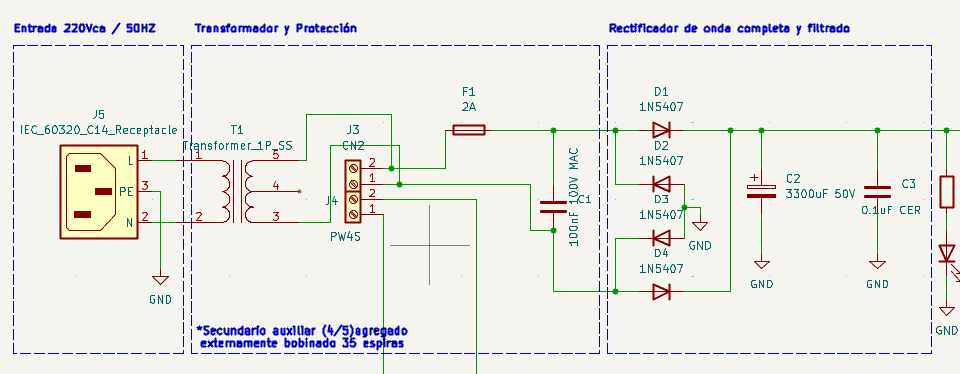
\includegraphics[
		width=\textwidth,
		keepaspectratio
		]{fuente_no_regulada.png}
		
		\caption{Circuito correspondiente a las etapas de transformación, rectificación y filtrado de la fuente de alimentación.}
		\label{fig:fuente_no_regulada}
	\end{figure}
	
	% ------------------------------------------------------------
	% TABLA DE MEDICIONES
	% ------------------------------------------------------------
	Los valores obtenidos durante el ensayo se registraron en la
	Tabla~\ref{tab:mediciones_no_regulada}.
	
	\begin{table}[H]
		\centering
		
		\caption{Mediciones sobre la fuente no regulada.}
		\label{tab:mediciones_no_regulada}
		
		\begin{tabular}{cc}
			
			\toprule
			
			\textbf{Corriente}
			&
			\textbf{Tensión DC}
		
			\\
			
			$I_L$ [A]
			&
			$V_{DC}$ [V]
			
		
			\\
			
			\midrule
			
			0    & 36,33  \\
			0,86 & 27  \\
			1,00 & 25,92  \\
			1,20 & 24,83  \\
			1,30 & 24,30  \\
			1,50 & 24,15  \\
			
			\bottomrule
			
		\end{tabular}
		
	\end{table}
	
	% ------------------------------------------------------------
	% EXPLICACIÓN DEL RIPPLE
	% ------------------------------------------------------------
	Al aumentar la corriente consumida por la carga, el capacitor de filtrado se
	descarga más rápidamente entre dos máximos consecutivos de la tensión
	rectificada. Como consecuencia, aumenta la amplitud del ripple.
	
	La tensión observada en el osciloscopio presenta aproximadamente la forma
	indicada en la Figura~\ref{fig:ripple_ensayo}.
	
	\begin{figure}[H]
		\centering
		
		\begin{tikzpicture}
			
			\begin{axis}[
				width=0.85\textwidth,
				height=5.5cm,
				xlabel={$t$},
				ylabel={$V(t)$},
				xmin=0,
				xmax=5,
				ymin=8,
				ymax=15,
				xtick=\empty,
				ytick=\empty,
				grid=both,
				axis lines=left
				]
				
				\addplot[
				thick
				]
				coordinates{
					(0,14)
					(0.9,11.8)
					(1,14)
					(1.9,11.8)
					(2,14)
					(2.9,11.8)
					(3,14)
					(3.9,11.8)
					(4,14)
					(4.9,11.8)
					(5,14)
				};
				
			\end{axis}
			
		\end{tikzpicture}
		
		\caption{Representación aproximada del ripple medido sobre el capacitor de
			filtrado.}
		\label{fig:ripple_ensayo}
		
	\end{figure}
	
	La tensión de ripple pico a pico se determina directamente a partir del
	osciloscopio mediante:
	
	\begin{equation}
		V_{r(pp)}
		=
		N_{\mathrm{div}}
		\cdot
		V_{\mathrm{div}},
	\end{equation}
	
	donde:
	
	\begin{itemize}
		\item $N_{\mathrm{div}}$ es la cantidad de divisiones verticales ocupadas
		por el ripple;
		
		\item $V_{\mathrm{div}}$ es la escala vertical seleccionada en el
		osciloscopio.
	\end{itemize}
	
	Para la condición de máxima carga se obtuvo:
	
	\begin{equation}
		V_{r(pp)}
		=
		2,5~\text{V}.
	\end{equation}
	
	% ------------------------------------------------------------
	% COMPARACIÓN CON VALOR TEÓRICO
	% ------------------------------------------------------------
	El valor teórico del ripple puede aproximarse mediante:
	
	\begin{equation}
		V_{r(pp)}
		\approx
		\frac{I_L}
		{f_{\mathrm{ripple}}C}.
	\end{equation}
	
	Como la rectificación es de onda completa:
	
	\begin{equation}
		f_{\mathrm{ripple}}
		=
		100~\text{Hz}.
	\end{equation}
	
	Para:
	
	\begin{align}
		I_L &= 1,5~\text{A},
		\\
		C &= 3300~\mu\text{F},
	\end{align}
	
	se obtiene:
	
	\begin{align}
		V_{r(pp)}
		&\approx
		\frac{1,5}
		{100(3300\times10^{-6})},
		\\
		V_{r(pp)}
		&\approx
		4,55~\text{V}.
	\end{align}
	
	Este valor será comparado con el obtenido experimentalmente para evaluar las
	diferencias entre el modelo teórico y el comportamiento real del circuito.
	
	% ============================================================
	% 2.1.2 RESISTENCIA INTERNA
	% ============================================================
	\subsubsection{Determinación de la resistencia interna del transformador y los diodos}
	
	La fuente no regulada puede modelarse mediante una fuente ideal de tensión
	$V_{\text{vacío}}$ conectada en serie con una resistencia interna equivalente
	$R_{\mathrm{int}}$.
	
	Esta resistencia representa principalmente los efectos de:
	
	\begin{itemize}
		
		\item la resistencia de los bobinados del transformador;
		
		\item las caídas de tensión producidas en los diodos;
		
		\item las pérdidas asociadas a las conexiones del circuito.
		
	\end{itemize}
	
	El circuito equivalente puede expresarse mediante:
	
	\begin{equation}
		V_{\text{carga}}
		=
		V_{\text{vacío}}
		-
		I_{\text{carga}}R_{\mathrm{int}}.
	\end{equation}
	
	Despejando la resistencia interna:
	
	\begin{equation}
		R_{\mathrm{int}}
		=
		\frac{
			V_{\text{vacío}}
			-
			V_{\text{carga}}
		}{
			I_{\text{carga}}
		}.
	\end{equation}
	
	Utilizando la condición de máxima carga:
	
	\begin{align}
		V_{\text{vacío}} &= 36,77~\text{V},
		\\
		V_{\text{carga}} &= 23,15~\text{V},
		\\
		I_{\text{carga}} &= 1,5~\text{A},
	\end{align}
	
	se obtiene:
	
	\begin{equation}
		R_{\mathrm{int}}
		=
		\frac{
			36,33
			-
			24,15
		}{
			1,5
		}
		=
		8,12\Omega.
	\end{equation}
	
	La existencia de esta resistencia interna explica por qué la tensión de la fuente
	no regulada disminuye al aumentar la corriente de carga.
	
	% ------------------------------------------------------------
	% GRÁFICO V-I
	% ------------------------------------------------------------
	A partir de los valores registrados puede construirse la curva
	$V_{\text{salida}}$ en función de $I_{\text{carga}}$.
	
	\begin{figure}[H]
	\centering
	
	\begin{tikzpicture}
		
		\begin{axis}[
			width=0.85\textwidth,
			height=7cm,
			xlabel={$I_{\text{carga}}$ [A]},
			ylabel={$V_{\text{salida}}$ [V]},
			xmin=0,
			xmax=1.6,
			ymin=23,
			ymax=38,
			xtick={0,0.2,0.4,0.6,0.8,1.0,1.2,1.4,1.6},
			ytick={24,26,28,30,32,34,36,38},
			grid=both,
			major grid style={line width=0.2pt},
			minor grid style={line width=0.1pt},
			tick label style={font=\small},
			label style={font=\small},
			]
			
			\addplot[
			thick,
			mark=*,
			mark size=2pt
			]
			coordinates{
				(0.00,36.33)
				(0.86,27.00)
				(1.00,25.92)
				(1.20,24.83)
				(1.30,24.30)
				(1.50,24.15)
			};
			
		\end{axis}
		
	\end{tikzpicture}
	
	\caption{Tensión de salida de la fuente no regulada en función de la corriente de carga.}
	\label{fig:vi_no_regulada}
	
	\end{figure}
		
	
	La pendiente negativa de esta curva permite visualizar el efecto de la
	resistencia interna equivalente de la fuente.
	
	% ============================================================
	% 2.2 MEDICIONES FINALES
	% ============================================================
	\subsection{Mediciones finales}
	
	Una vez incorporada la etapa de regulación con el LM317 se realizaron los
	ensayos finales de la fuente.
	
	Las mediciones se efectuaron tanto en condición de vacío como a máxima carga,
	con el objetivo de analizar la capacidad del regulador para mantener estable la
	tensión de salida.
	
	% ============================================================
	% 2.2.1 REGULACIÓN DE VOLTAJE
	% ============================================================
	\subsubsection{Regulación de voltaje}
	
	La regulación de voltaje permite cuantificar cuánto varía la tensión de salida
	entre la condición sin carga y la condición de carga máxima.
	
	Se calcula mediante:
	
	\begin{equation}
		RV
		=
		\frac{
			V_{\text{vacío}}
			-
			V_{\text{carga}}
		}{
			V_{\text{carga}}
		}
		\times 100\%.
	\end{equation}
	
	Los valores medidos fueron:
	
	\begin{align}
		V_{\text{vacío}}
		&=
		30,66\text{V},
		\\
		V_{\text{carga}}
		&=
		15,77\text{V},
		\\
		I_{\text{carga}}
		&=
		1,5~\text{A}.
	\end{align}
	
	Por lo tanto:
	
	\begin{equation}
		RV
		=
		\frac{
			30,66
			-
			15,77
		}{
			15,77
		}
		\times 100\%
		=
		48,56
	\end{equation}
	
	Cuanto menor sea este porcentaje, menor será la variación de la tensión de
	salida frente a cambios de carga y, por lo tanto, mejor será la regulación de la
	fuente.
	
	% ============================================================
	% 2.2.2 FACTOR DE RIPPLE
	% ============================================================
	\subsubsection{Factor de ripple}
	
	El factor de ripple permite expresar la magnitud de la componente alterna
	residual respecto de la componente continua de la tensión de salida.
	
	Se define como:
	
	\begin{equation}
		FR
		=
		\frac{
			V_{r(\mathrm{rms})}
		}{
			V_{DC}
		}
		\times 100\%.
	\end{equation}
	
	Si el ripple observado puede aproximarse mediante una señal triangular, su valor
	eficaz se relaciona con el valor pico a pico mediante:
	
	\begin{equation}
		V_{r(\mathrm{rms})}
		=
		\frac{
			V_{r(pp)}
		}{
			2\sqrt{3}
		}.
	\end{equation}
	
	El ripple medido a la salida del regulador fue:
	
	\begin{equation}
		V_{r(pp)}
		=
		2m\text{V}.
	\end{equation}
	
	Por lo tanto:
	
	\begin{equation}
		V_{r(\mathrm{rms})}
		=
		\frac{
			0,002
		}{
			2\sqrt{3}
		}
		=
		0,577\text{V}.
	\end{equation}
	
	Considerando una tensión continua de salida de:
	
	\begin{equation}
		V_{DC}
		=
		\dato[2cm]~\text{V},
	\end{equation}
	
	el factor de ripple resulta:
	
	\begin{equation}
		FR
		=
		\frac{
			\dato[1.5cm]
		}{
			\dato[1.5cm]
		}
		\times 100\%
		=
		\dato[2cm]\%.
	\end{equation}
	
	El regulador LM317 reduce considerablemente la componente de ripple presente a su
	entrada, siempre que se mantenga dentro de su región normal de regulación.
	
	% ============================================================
	% 2.2.3 TEMPERATURA DE JUNTURA
	% ============================================================
	\subsubsection{Cálculo de la temperatura de juntura}
	
	Debido a que el LM317 es un regulador lineal, la diferencia entre la tensión de
	entrada y la tensión de salida se disipa principalmente en forma de calor.
	
	La potencia disipada por el regulador puede aproximarse mediante:
	
	\begin{equation}
		P_D
		=
		(V_{IN}-V_O)I_O.
	\end{equation}
	
	Para las condiciones del ensayo:
	
	\begin{align}
		V_{IN} &= \dato[2cm]~\text{V},
		\\
		V_O &= \dato[2cm]~\text{V},
		\\
		I_O &= 1,5~\text{A},
	\end{align}
	
	la potencia disipada resulta:
	
	\begin{equation}
		P_D
		=
		\left(
		\dato[1.5cm]
		-
		\dato[1.5cm]
		\right)
		(1,5)
		=
		\dato[2cm]~\text{W}.
	\end{equation}
	
	Durante el ensayo se midió la temperatura de carcasa del LM317:
	
	\begin{equation}
		T_C
		=
		\dato[2cm]~^\circ\text{C}.
	\end{equation}
	
	Conociendo la resistencia térmica entre la juntura y la carcasa
	$\theta_{JC}$, obtenida de la hoja de datos, la temperatura de juntura puede
	estimarse mediante:
	
	\begin{equation}
		T_J
		=
		T_C
		+
		P_D\theta_{JC}.
	\end{equation}
	
	Reemplazando los valores:
	
	\begin{equation}
		T_J
		=
		\dato[1.5cm]
		+
		\left(
		\dato[1.5cm]
		\right)
		\left(
		\dato[1.5cm]
		\right)
		=
		\dato[2cm]~^\circ\text{C}.
	\end{equation}
	
	El valor obtenido debe compararse con la temperatura máxima de juntura indicada
	por el fabricante para verificar que el regulador opere dentro de condiciones
	térmicas seguras.
	
	% ============================================================
	% 3. CONCLUSIONES
	% ============================================================
	\newpage
	\section{Conclusiones}
	
	A partir de los ensayos realizados fue posible verificar experimentalmente el
	funcionamiento de las distintas etapas que componen la fuente de alimentación.
	
	En la fuente no regulada se observó que, al aumentar la corriente de carga, la
	tensión continua de salida disminuye como consecuencia de la resistencia interna
	equivalente del transformador, los diodos y las conexiones. Simultáneamente,
	aumenta la amplitud del ripple debido a la mayor descarga del capacitor entre
	los máximos de la señal rectificada.
	
	La incorporación del regulador LM317 permitió mejorar considerablemente la
	estabilidad de la tensión de salida y reducir el ripple presente en la carga.
	
	La regulación de voltaje obtenida experimentalmente fue de:
	
	\begin{equation}
		RV
		=
		\dato[2cm]\%.
	\end{equation}
	
	mientras que el factor de ripple a la salida resultó:
	
	\begin{equation}
		FR
		=
		\dato[2cm]\%.
	\end{equation}
	
	Finalmente, el análisis térmico permitió estimar una temperatura de juntura de:
	
	\begin{equation}
		T_J
		=
		\dato[2cm]~^\circ\text{C},
	\end{equation}
	
	permitiendo evaluar si el sistema de disipación utilizado resulta adecuado para
	el funcionamiento de la fuente a máxima carga.
	
	En función de los resultados obtenidos se podrá determinar si la fuente cumple
	con las especificaciones de diseño de tensión variable y corriente máxima
	establecidas para el trabajo práctico.
	
% ============================================================
% ANEXO
% ============================================================
\newpage
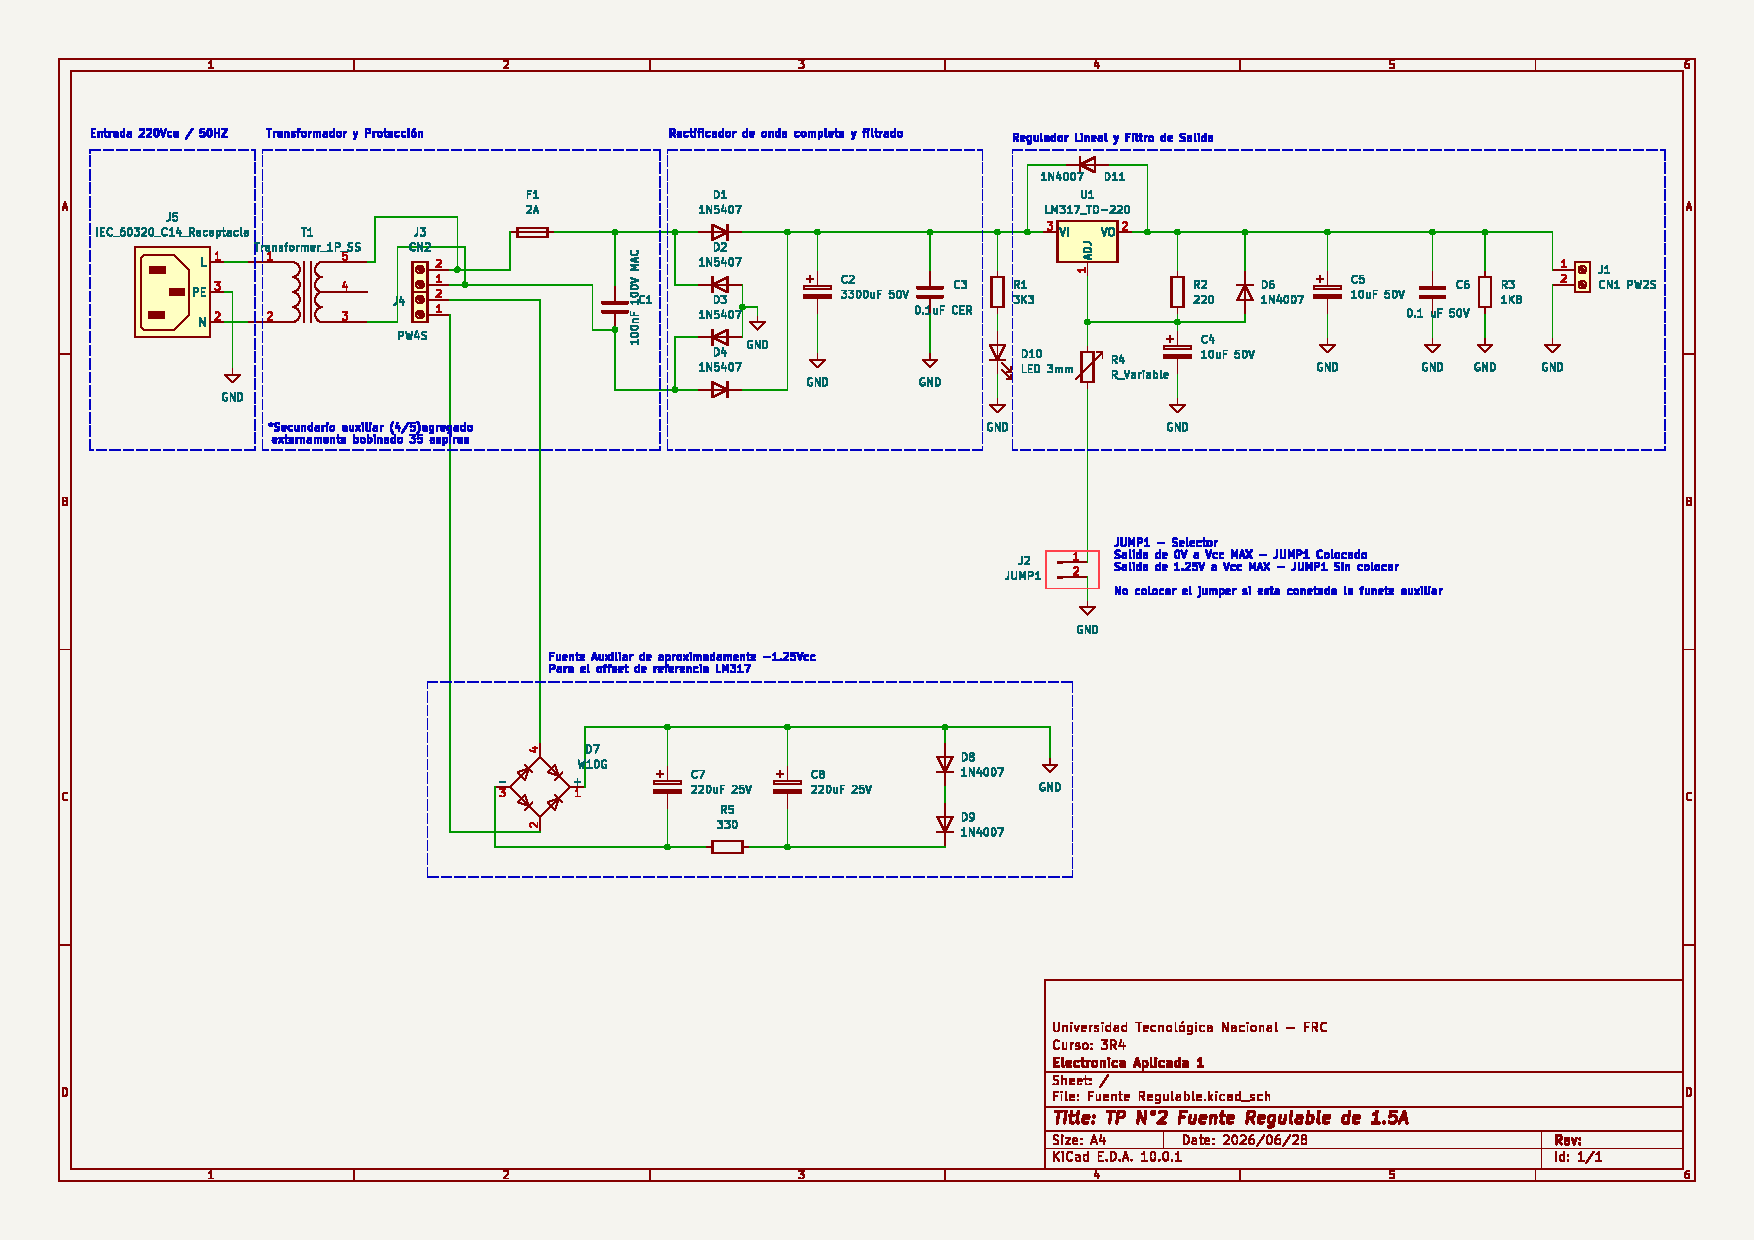
\includepdf[
pages=1,
scale=0.8,
angle=90,
pagecommand={
      \section{Esquemático completo de la fuente}             
                   }
]{Fuente regulable.pdf}
	
	% ============================================================
	% BIBLIOGRAFÍA
	% ============================================================
	\newpage
	\section{Bibliografía}
	
	\begin{thebibliography}{9}
		
		\bibitem{guia}
		Universidad Tecnológica Nacional, Facultad Regional Córdoba,
		\textit{Guía de ejercicios N.º 1: Fuentes de alimentación},
		Electrónica Aplicada I.
		
		\bibitem{diapositivas}
		Universidad Tecnológica Nacional, Facultad Regional Córdoba,
		\textit{Fuentes de Alimentación},
		Electrónica Aplicada I.
		
		\bibitem{lm317}
		Hoja de datos del regulador de tensión ajustable LM317.
		
	\end{thebibliography}
	
	
	% ============================================================
	% FIN DEL DOCUMENTO
	% ============================================================
\end{document}